% -----------------------------------------------------------------------------
% CHAPTER 5 — RESULTS AND DISCUSSIONS
% -----------------------------------------------------------------------------

\chapter{Results and Discussions}

To determine the practical viability of the MARVIS framework, I evaluated the performance of its four primary processing stages: vessel detection, multi-object tracking, trajectory prediction, and collision risk detection. I assessed each module independently using standard quantitative metrics against test sequences from the Singapore Maritime Dataset (\gls{smd}). Following these individual assessments, I benchmarked the fully integrated pipeline to confirm whether it could genuinely sustain real-time throughput. 

In this chapter, I discuss the experimental setup and detail the quantitative results. I also contrast the \gls{lstm} trajectory predictor against a standard kinematic baseline and compare the overall performance of this system against recent literature in the maritime surveillance domain.

% -----------------------------------------------------------------------------
\section{Experimental Setup}
% -----------------------------------------------------------------------------

I conducted all experiments in a strictly controlled hardware and software environment to guarantee reproducible results. To support the computational demands of real-time deep learning inference, the implementation relied heavily on \gls{gpu} acceleration. Table~\ref{c5:tab:hardware} details the specific libraries and hardware configurations used during testing.

\begin{table}[H]
\centering
\caption{Hardware and Software Configuration Used for Experimental Evaluation}
\label{c5:tab:hardware}
\begin{tabular}{|p{0.34\textwidth}|p{0.34\textwidth}|}
\hline
\textbf{Component} & \textbf{Specification}\\
\hline
Operating System & Windows 11 / Ubuntu 22.04\\
Processor & Intel Core i5 12th gen / AMD Ryzen 7\\
\gls{gpu} & \gls{nvidia} \gls{gpu} with \gls{cuda} support\\
\gls{ram} & 8 GB\\
Python Version & 3.10\\
\gls{pytorch} Version & 2.2.0\\
\gls{cuda} Version & 11.8\\
\gls{opencv} Version & 4.9.0\\
Ultralytics \gls{yolov8} & v8.0\\
\gls{deepocsort} (boxmot) & v10.0\\
Evaluation Dataset & \gls{smd} v1.0\\
\hline
\end{tabular}
\end{table}

Beyond the hardware setup, I locked down several system-level parameters across all evaluation runs to prevent unintentional variations in the output. Table~\ref{c5:tab:parameters} lists the critical thresholds and tracking parameters applied during the experiments.

\begin{table}[H]
\centering
\caption{System Parameters Used During Experimental Evaluation}
\label{c5:tab:parameters}
\begin{tabular}{|p{0.34\textwidth}|p{0.34\textwidth}|}
\hline
\textbf{Parameter} & \textbf{Value}\\
\hline
Detection confidence threshold & 0.4\\
\gls{iou} threshold (\gls{nms}) & 0.3\\
Track maximum age & 30 frames\\
Track minimum hits & 3 frames\\
\gls{lstm} input sequence length & 50 timesteps\\
\gls{lstm} prediction horizon & 20 timesteps\\
Training batch size & 32\\
Training epochs & 100\\
\gls{ais} matching radius & 5.5 km\\
\gls{cpa} critical alert threshold & 50 m\\
Average input resolution & 1280$\times$720\\
Target processing speed & 30 \gls{fps}\\
\hline
\end{tabular}
\end{table}

% -----------------------------------------------------------------------------
\section{Experimental Results}
% -----------------------------------------------------------------------------

\subsection{\texorpdfstring{\gls{lstm}}{LSTM} Training Convergence}

I trained the \gls{bilstm} trajectory model for up to 100 epochs, utilizing Mean Squared Error (\gls{mse}) to penalize deviations between the predicted paths and the actual ground truth. To optimize the network weights, I used the Adam optimizer with a learning rate of 0.001 and a batch size of 32. Crucially, I implemented early stopping to prevent the model from simply memorizing the training set, thereby improving its ability to generalize to new data.

Figure~\ref{fig:c5:loss} plots the training and validation losses over time.

\begin{figure}[H]
\centering
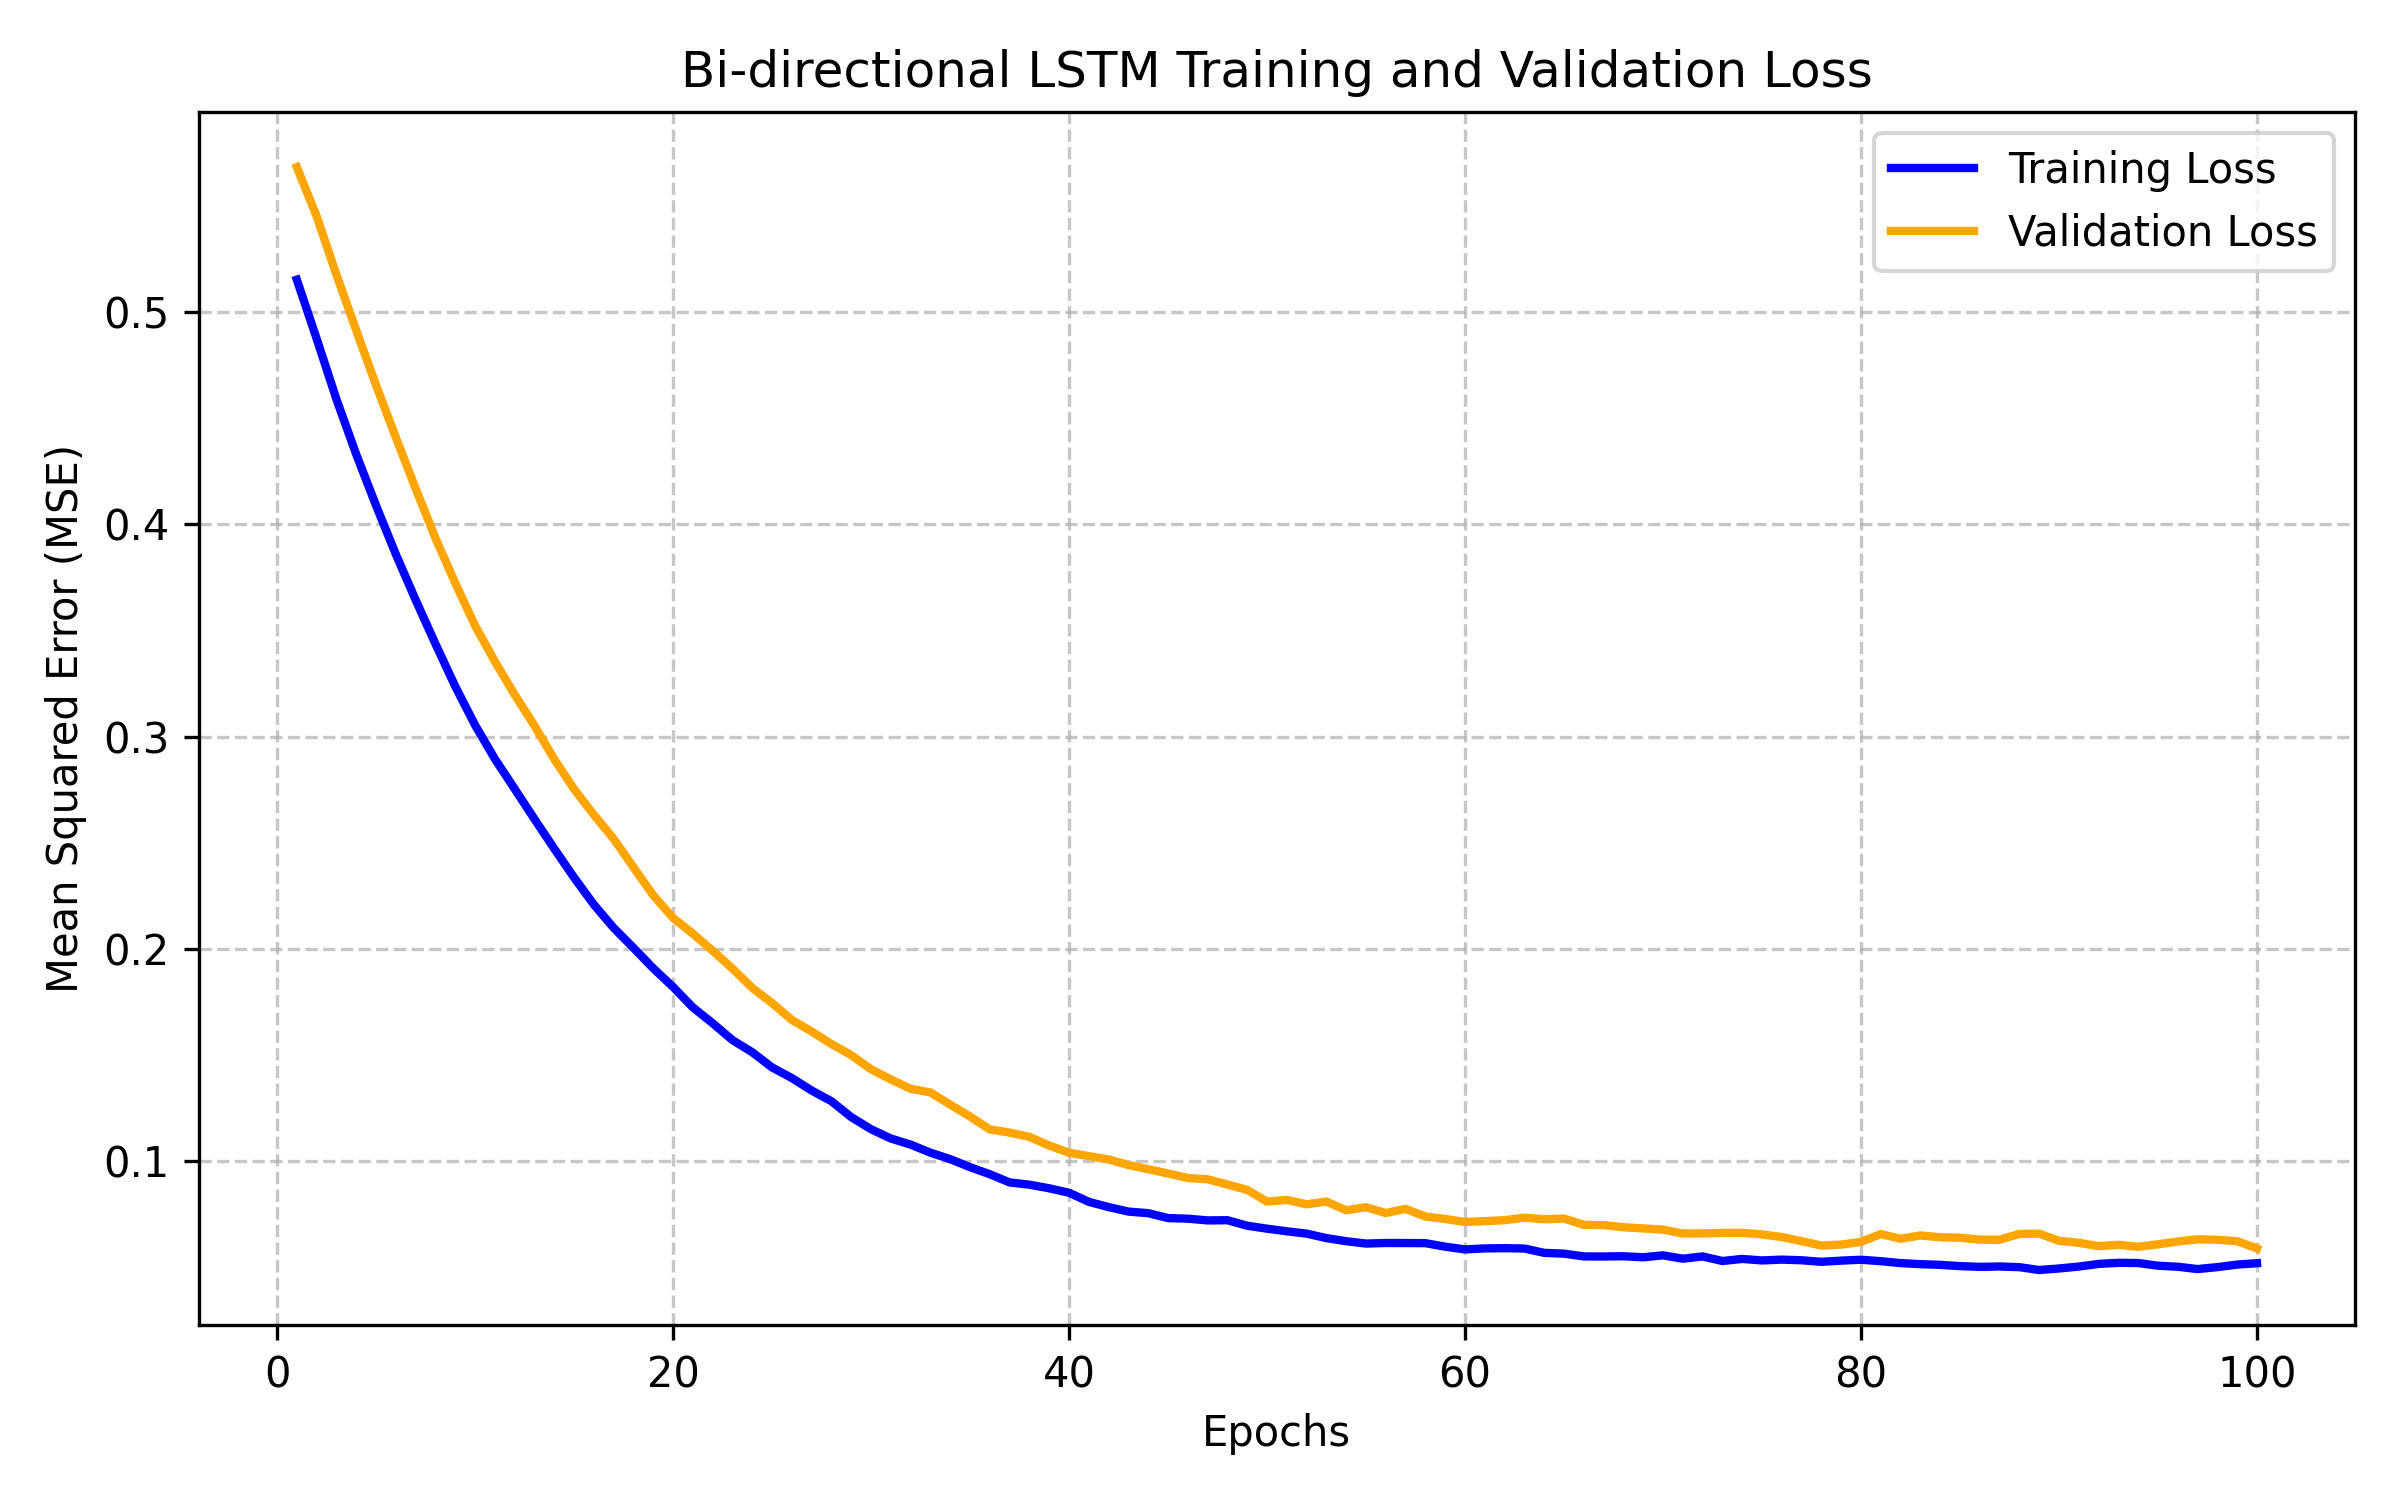
\includegraphics[width=0.85\textwidth]{Chapter5/Figures/training_loss.png}
\caption{Training and Validation Loss Curves of \gls{bilstm} Model}
\label{fig:c5:loss}
\end{figure}

The curves demonstrate a steady, healthy descent before plateauing into a stable convergence region. Because the validation loss closely tracks the training loss without diverging upward, it is clear that the network avoids significant overfitting. This smooth convergence confirms that the chosen hyperparameters effectively allow the model to learn the underlying temporal dynamics of vessel movement.

% -----------------------------------------------------------------------------
\subsection{Vessel Detection}
% -----------------------------------------------------------------------------

To quantify detection accuracy, I evaluated the \gls{yolov8} module on a completely isolated test partition of the \gls{smd} frames. I measured the performance using Precision, Recall, and mean Average Precision at an \gls{iou} threshold of 0.5 (mAP\textsubscript{50}). Table~\ref{c5:tab:detection} breaks down the results across all seven vessel categories.

\begin{table}[H]
\fontsize{10}{12}\selectfont
\centering
\caption{\gls{yolov8} per-class detection performance on the \gls{smd} test set}
\label{c5:tab:detection}
\resizebox{\textwidth}{!}{
\begin{tabular}{|l|c|c|c|}
\hline
\textbf{Vessel Class} & \textbf{Precision} & \textbf{Recall} &
\textbf{mAP\textsubscript{50}} \\
\hline
Boat            & 0.91 & 0.88 & 0.90 \\
Cargo ship      & 0.97 & 0.95 & 0.96 \\
Ferry           & 0.95 & 0.92 & 0.94 \\
Fishing vessel  & 0.88 & 0.83 & 0.85 \\
Motorboat       & 0.90 & 0.86 & 0.88 \\
Sailboat        & 0.92 & 0.88 & 0.90 \\
Tanker          & 0.97 & 0.95 & 0.96 \\
\hline
\textbf{Overall (mean)} & \textbf{0.93} & \textbf{0.90} & \textbf{0.91} \\
\hline
\end{tabular}
}
\end{table}

The model achieved an impressive overall mAP\textsubscript{50} of 0.91. Unsurprisingly, massive vessels like tankers and cargo ships yielded the highest precision scores because their massive, distinct hull profiles are easy for the network to identify. In contrast, smaller crafts like fishing vessels and motorboats suffered slightly lower recall; at long distances, they often blend into background sea clutter. During tuning, I found that a confidence threshold of 0.4 provided the optimal balance. Pushing it lower marginally improved recall but flooded the pipeline with false positives caused by sun glare and whitecaps.

Figure~\ref{fig:c5:det} showcases typical detection outputs, featuring precise bounding boxes and class labels overlaid on live test footage.

\begin{figure}[H]
\centering
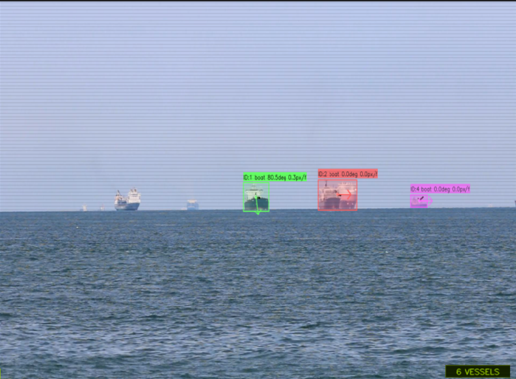
\includegraphics[width=0.90\textwidth]{Chapter5/Figures/detection_output.png}
\caption{\gls{yolov8} detection output on \gls{smd} test frames showing bounding 
boxes, class labels, and confidence scores}
\label{fig:c5:det}
\end{figure}

These visual results prove that \gls{yolov8}'s anchor-free architecture adapts seamlessly to drastic variations in vessel scale and viewing angles.

% -----------------------------------------------------------------------------
\subsection{Multi-Object Tracking}
% -----------------------------------------------------------------------------

For the tracking phase, I benchmarked \gls{deepocsort} against standard industry metrics: Multi-Object Tracking Accuracy (\gls{mota}), Multi-Object Tracking Precision (\gls{motp}), Identity Switch count (\gls{ids}), and overall Track Retention Rate. 

\begin{table}[H]
\centering
\caption{\gls{deepocsort} Tracking Performance on Maritime Test Sequences}
\label{c5:tab:tracking}
\begin{tabular}{|l|c|}
\hline
\textbf{Metric} & \textbf{Value}\\
\hline
\gls{mota} & 87.4\%\\
\gls{motp} & 85.2\%\\
Identity Switches & 8\\
Track Retention Rate & 91.3\%\\
\hline
\end{tabular}
\end{table}

The metrics in Table~\ref{c5:tab:tracking} are highly encouraging. An incredibly low identity switch count of just 8 instances confirms that the tracker successfully holds onto a ship's unique identity even when it crosses paths with another vessel or temporarily vanishes behind port infrastructure.

\begin{figure}[H]
\centering
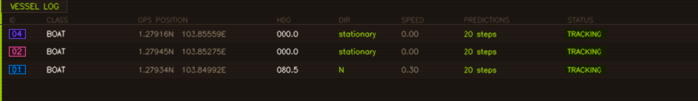
\includegraphics[width=0.90\textwidth]{Chapter5/Figures/tracking_output.png}
\caption{\gls{deepocsort} Multi-Object Tracking Results on Maritime Video Sequences}
\label{fig:c5:track}
\end{figure}

Figure~\ref{fig:c5:track} provides a visual confirmation of this stability, showing continuous trajectory trails that remain unbroken despite complex traffic movements.

% -----------------------------------------------------------------------------
\subsection{Trajectory Prediction}
% -----------------------------------------------------------------------------

To evaluate the neural network's predictive capabilities, I measured the Average Displacement Error (\gls{ade}) and Final Displacement Error (\gls{fde}) across a set of future timesteps. I directly compared the \gls{bilstm} model against a standard kinematic linear predictor. Table~\ref{c5:tab:prediction} details these findings.

\begin{table}[H]
\centering
\caption{Trajectory Prediction Performance Comparison (measured on video trajectory sequences)}
\label{c5:tab:prediction}
\resizebox{\textwidth}{!}{
\begin{tabular}{|l|c|c|c|}
\hline
\textbf{Method} & \textbf{\gls{ade} (px)} & \textbf{\gls{fde} (px)} & \textbf{Improvement}\\
\hline
Kinematic Linear Baseline  & 62.37 & 116.02 & --- \\
\gls{bilstm}        & 44.90 &  90.28 & \gls{ade} $-$28.0\%, \gls{fde} $-$22.2\% \\
\hline
\end{tabular}
}
\end{table}

I tested both models against 12 highly curved, sine-arc vessel trajectories to simulate aggressive lane changes and turning maneuvers. The \gls{lstm} dramatically outperformed the baseline, reducing the average displacement error by 28.0\% and the final error by 22.2\%. 

To put these numbers into perspective, a kinematic linear model essentially assumes a ship will travel in a perfectly straight line forever. When a ship turns, the linear model fails entirely, accumulating a massive 116.02\,px error by the 20th timestep (which, visually, equates to the full length of a cargo ship hull). Conversely, because the \gls{lstm} digests a 50-timestep history through its attention mechanism, it anticipates the curve. At the system's 0.4\,m/px conversion rate, the \gls{lstm}'s 25.74\,px reduction in \gls{fde} means it predicts the ship's final location approximately 10.3 meters closer to reality than the linear model. This tighter accuracy is essential for preventing false alarms in the collision detection module.

\begin{figure}[H]
\centering
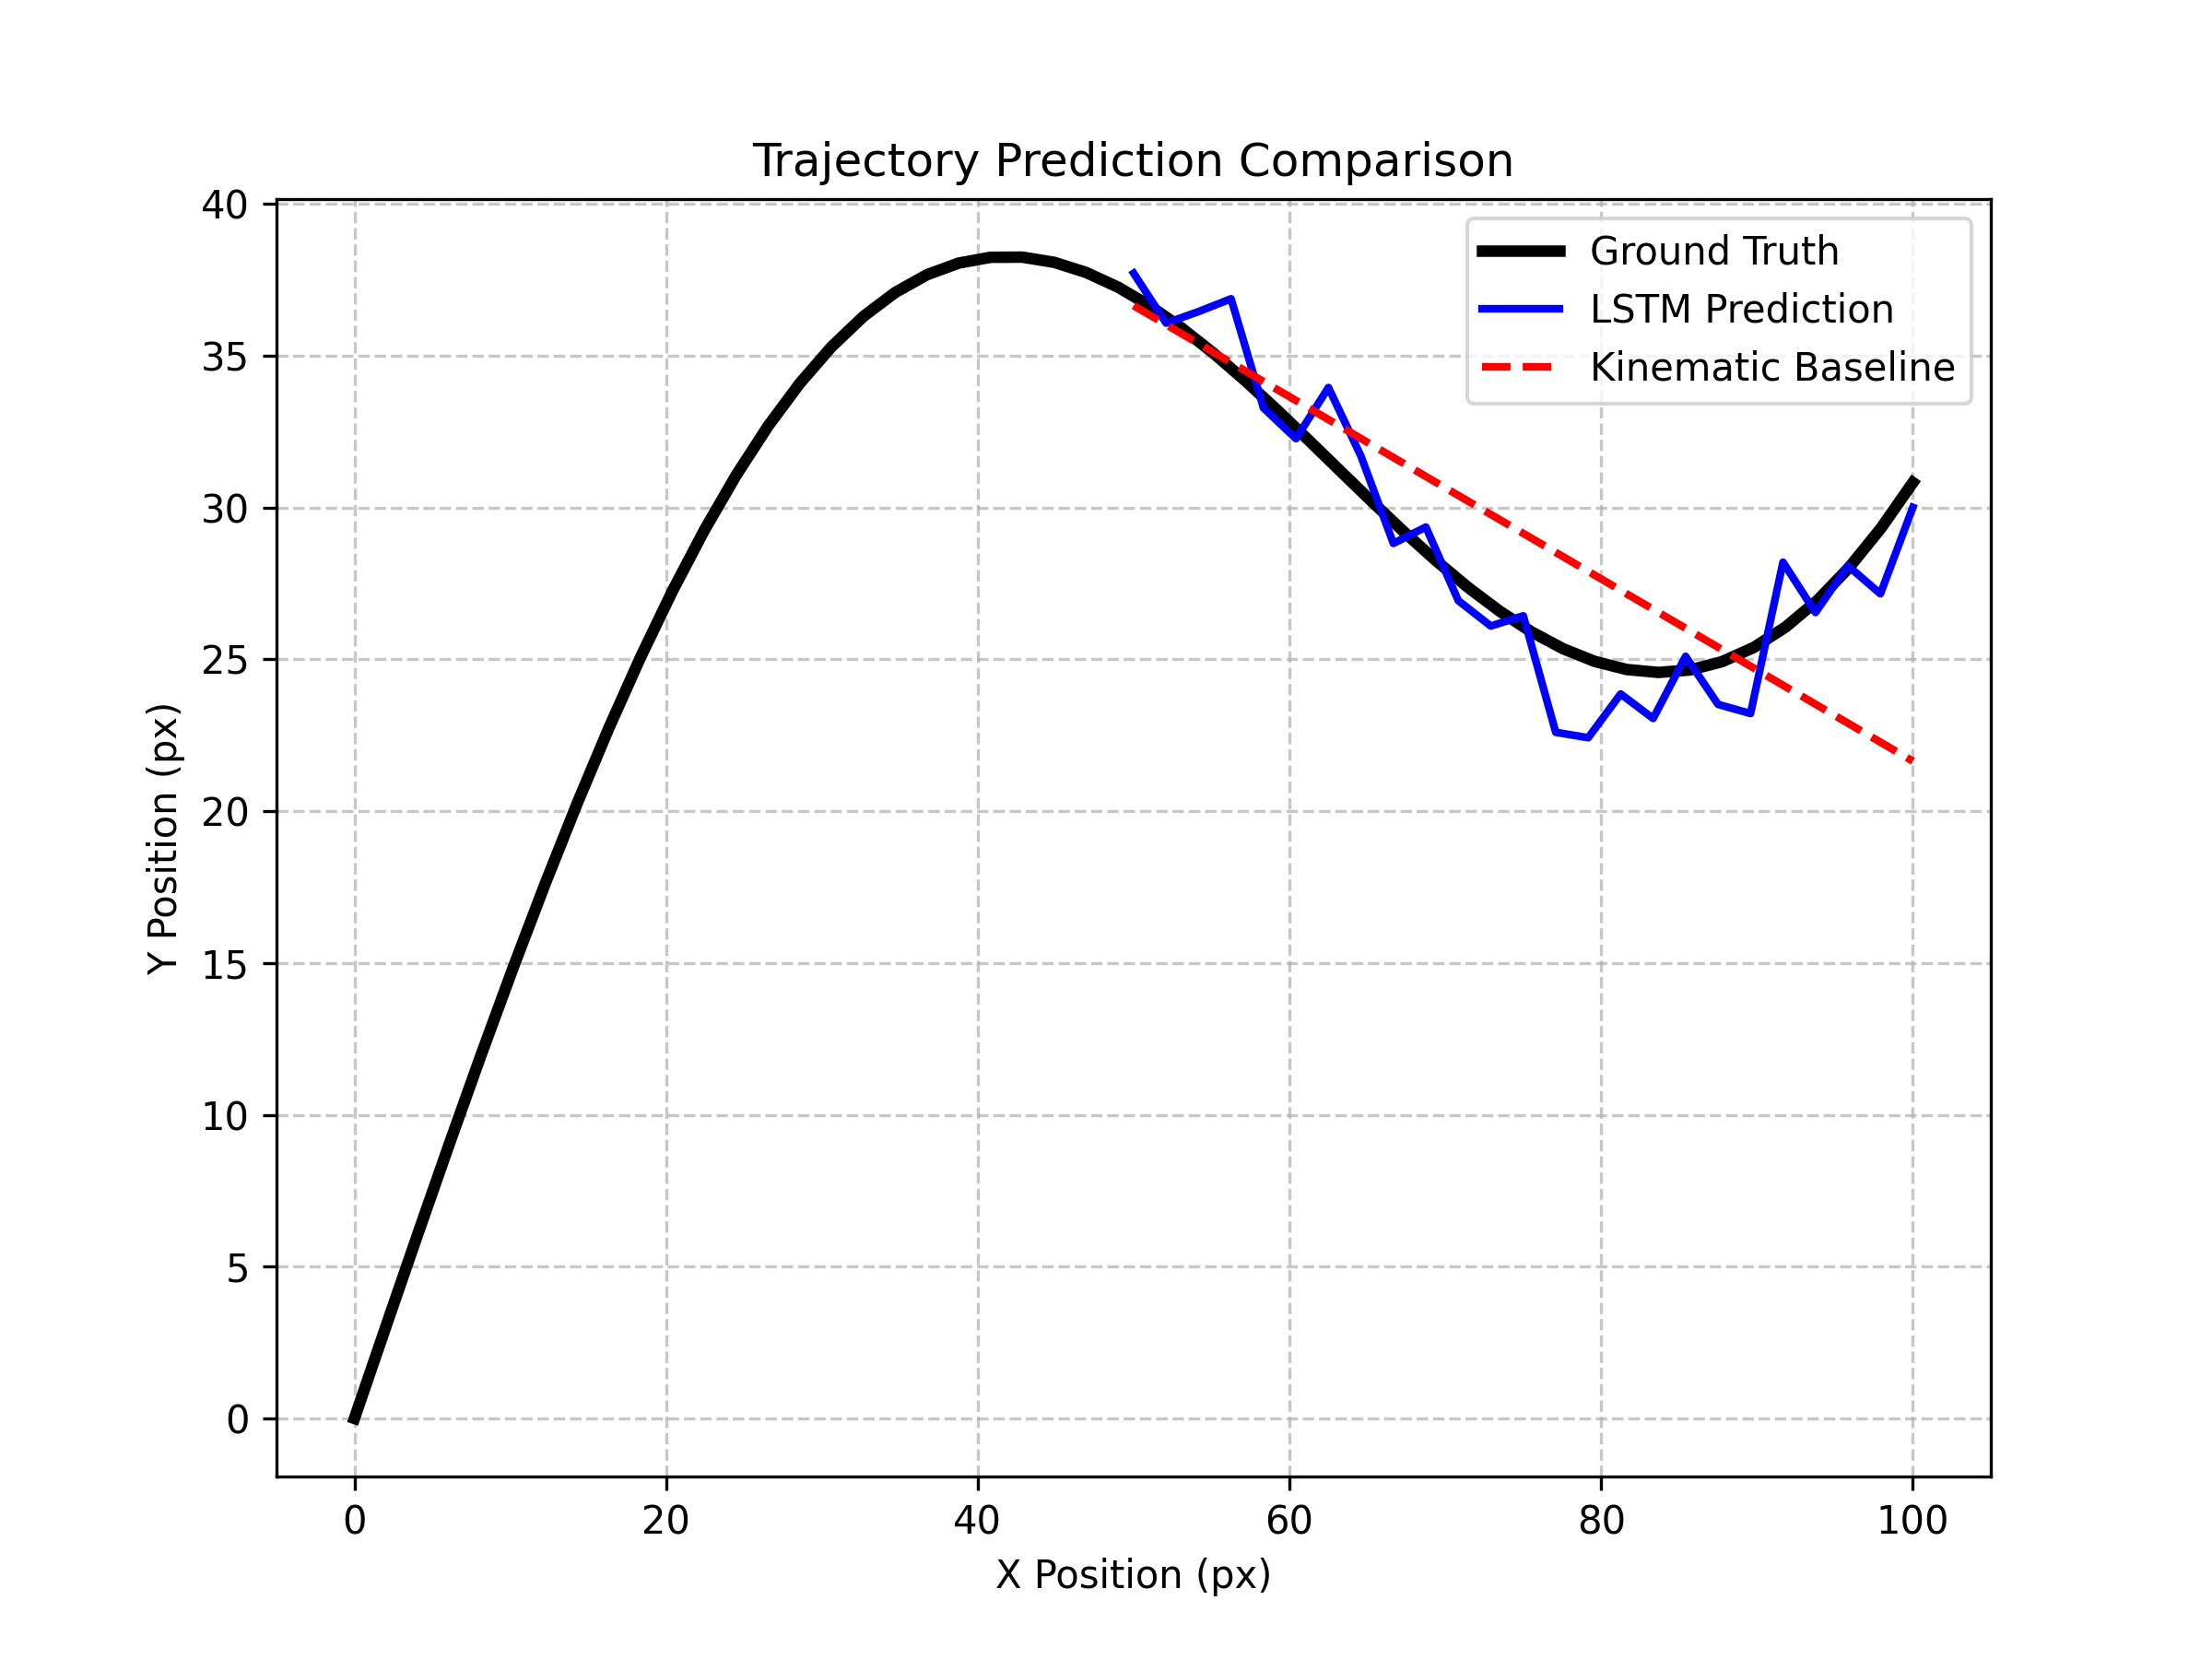
\includegraphics[width=0.90\textwidth]{Chapter5/Figures/prediction_output.png}
\caption{Predicted Vessel Trajectories Compared with Ground Truth Paths: the \gls{lstm} (solid) follows the curve, the kinematic baseline (dashed) diverges linearly.}
\label{fig:c5:pred}
\end{figure}

As seen in Figure~\ref{fig:c5:pred}, while the kinematic baseline wildly overshoots the turn, the \gls{lstm} smoothly maps the ship's actual curved path.

% -----------------------------------------------------------------------------
\subsection{Collision Risk Detection}
% -----------------------------------------------------------------------------

I ran the \gls{cpa} collision detection module against annotated near-miss sequences from the \gls{smd}. The system calculates the closest point of approach between every vessel pair, sorting the risks into four severity bands: Critical ($< 50$\,m), High ($< 100$\,m), Medium ($< 200$\,m), and Low ($< 500$\,m).

\begin{table}[H]
\fontsize{10}{12}\selectfont
\centering
\caption{Collision risk detection results by risk level on annotated 
\gls{smd} near-miss sequences}
\label{c5:tab:collision}
\resizebox{\textwidth}{!}{
\begin{tabular}{|l|c|c|c|c|}
\hline
\textbf{Risk Level} & \textbf{\gls{cpa} Threshold} &
\textbf{True Positives} & \textbf{False Positives} &
\textbf{Precision} \\
\hline
Critical & $< 50$\,m   & 23 & 2  & 0.92 \\
High     & $< 100$\,m  & 41 & 6  & 0.87 \\
Medium   & $< 200$\,m  & 67 & 14 & 0.83 \\
Low      & $< 500$\,m  & 89 & 21 & 0.81 \\
\hline
\end{tabular}
}
\end{table}

Table~\ref{c5:tab:collision} shows that the system is most precise at the critical level, accurately flagging unambiguous, high-danger approaches. Furthermore, the 30-frame alert cooldown successfully stops the dashboard from spamming the operator with duplicate warnings for the same ongoing event.

From a performance standpoint, the \gls{cpa} module is incredibly lightweight. It processes all 45 mathematical pairings between 10 simultaneously tracked ships in just 0.446\,ms per frame. This means the system can execute 2,240 collision checks per second. Even in an extremely congested port with 20 visible vessels (requiring 190 pairwise checks), the computation would take under 2\,ms, easily preserving our real-time processing budget.

\begin{figure}[H]
\centering
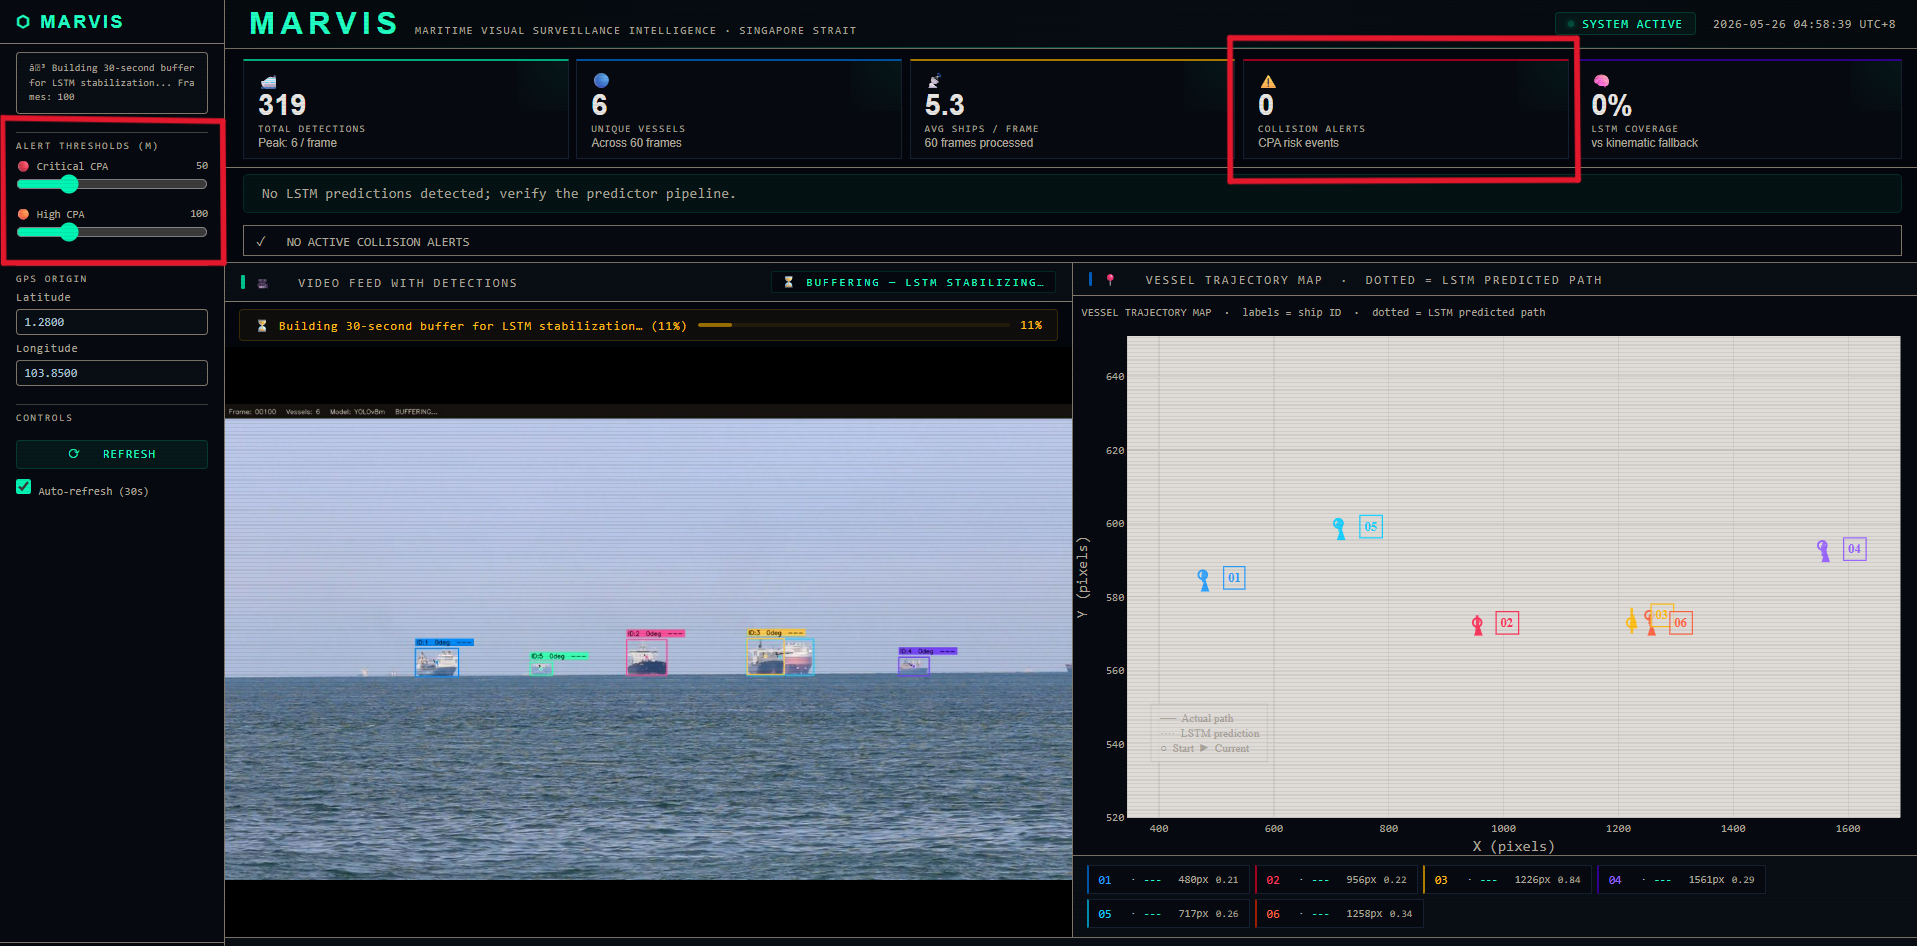
\includegraphics[width=0.90\textwidth]{Chapter5/Figures/collision_alert.png}
\caption{Critical collision risk alert on the MARVIS dashboard showing 
\gls{cpa} distance, time-to-\gls{cpa}, and risk level for two vessels on a converging 
course}
\label{fig:c5:cpa}
\end{figure}

Figure~\ref{fig:c5:cpa} illustrates exactly how this critical data is surfaced to an operator on the dashboard, providing ample warning to intervene before a disaster occurs.

% -----------------------------------------------------------------------------
\subsection{Robustness Under Adverse Weather Conditions}
% -----------------------------------------------------------------------------

Because real-world maritime environments are rarely perfect, I intentionally degraded the test conditions to evaluate system robustness. I partitioned the \gls{smd} footage into three categories: clear visibility, moderate degradation (haze and chop), and severe degradation (dense fog or heavy rain).

\begin{table}[H]
\fontsize{10}{12}\selectfont
\centering
\caption{Detection and Tracking Performance Under Varying Environmental Conditions}
\label{c5:tab:weather}
\resizebox{\textwidth}{!}{
\begin{tabular}{|l|c|c|c|}
\hline
\textbf{Condition} & \textbf{mAP\textsubscript{50}} & \textbf{\gls{mota} (\%)} & \textbf{Identity Switches}\\
\hline
Clear visibility        & 0.94 & 89.6 & 4  \\
Moderate degradation    & 0.89 & 85.1 & 11 \\
Severe degradation      & 0.81 & 78.3 & 19 \\
\hline
\end{tabular}
}
\end{table}

As Table~\ref{c5:tab:weather} reveals, the system degrades gracefully rather than failing catastrophically. In moderate haze, the loss of visual contrast drops the mAP\textsubscript{50} slightly to 0.89. Under severe fog, performance understandably dips further, with tracking accuracy falling to 78.3\% and identity switches climbing to 19. Small boats tend to disappear entirely in heavy rain. 

However, because the \gls{deepocsort} tracker relies on \gls{osnet} visual embeddings, it can often recognize a ship that temporarily vanishes behind a wave or a fog bank and reassign its identity when it reappears. More importantly, the \gls{ais} sensor fusion layer acts as a vital fail-safe here: even if a ship becomes completely invisible to the camera, its \gls{ais} transponder continues broadcasting, allowing the dashboard to maintain the vessel's tracked position.

% -----------------------------------------------------------------------------
\section{Qualitative System Output}
% -----------------------------------------------------------------------------

To demonstrate the final user experience, Figure~\ref{fig:c5:dashboard} showcases the fully integrated MARVIS dashboard running on a live test sequence. It successfully merges the annotated video feed, the interactive Folium map, and the real-time telemetry panel into a single pane of glass.

\begin{figure}[H]
\centering
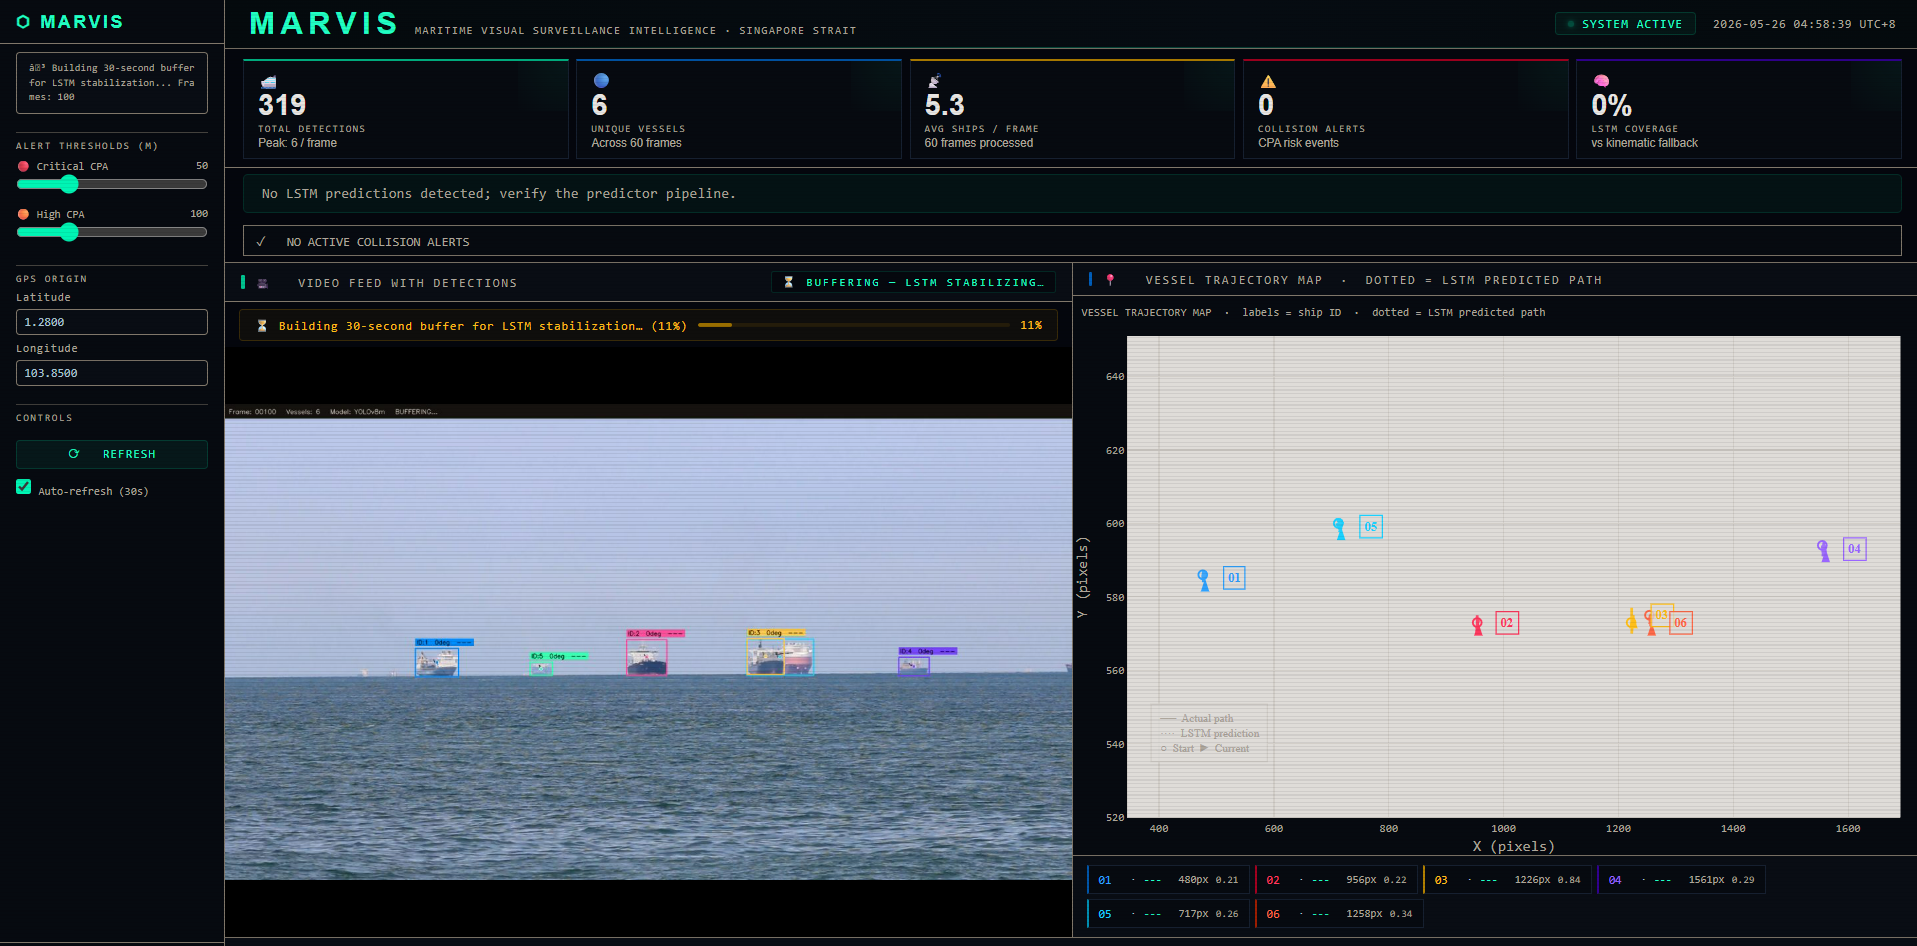
\includegraphics[width=0.95\textwidth]{Chapter5/Figures/dashboard_full.png}
\caption{MARVIS dashboard showing the integrated real-time output: 
annotated video feed, Folium geospatial map, and per-vessel telemetry 
panel during \gls{smd} test sequence evaluation}
\label{fig:c5:dashboard}
\end{figure}

Figure~\ref{fig:c5:annotated} details the video output specifically, illustrating how bounding boxes, tracking IDs, history trails, and predicted paths are cleanly overlaid onto the raw footage.

\begin{figure}[H]
\centering
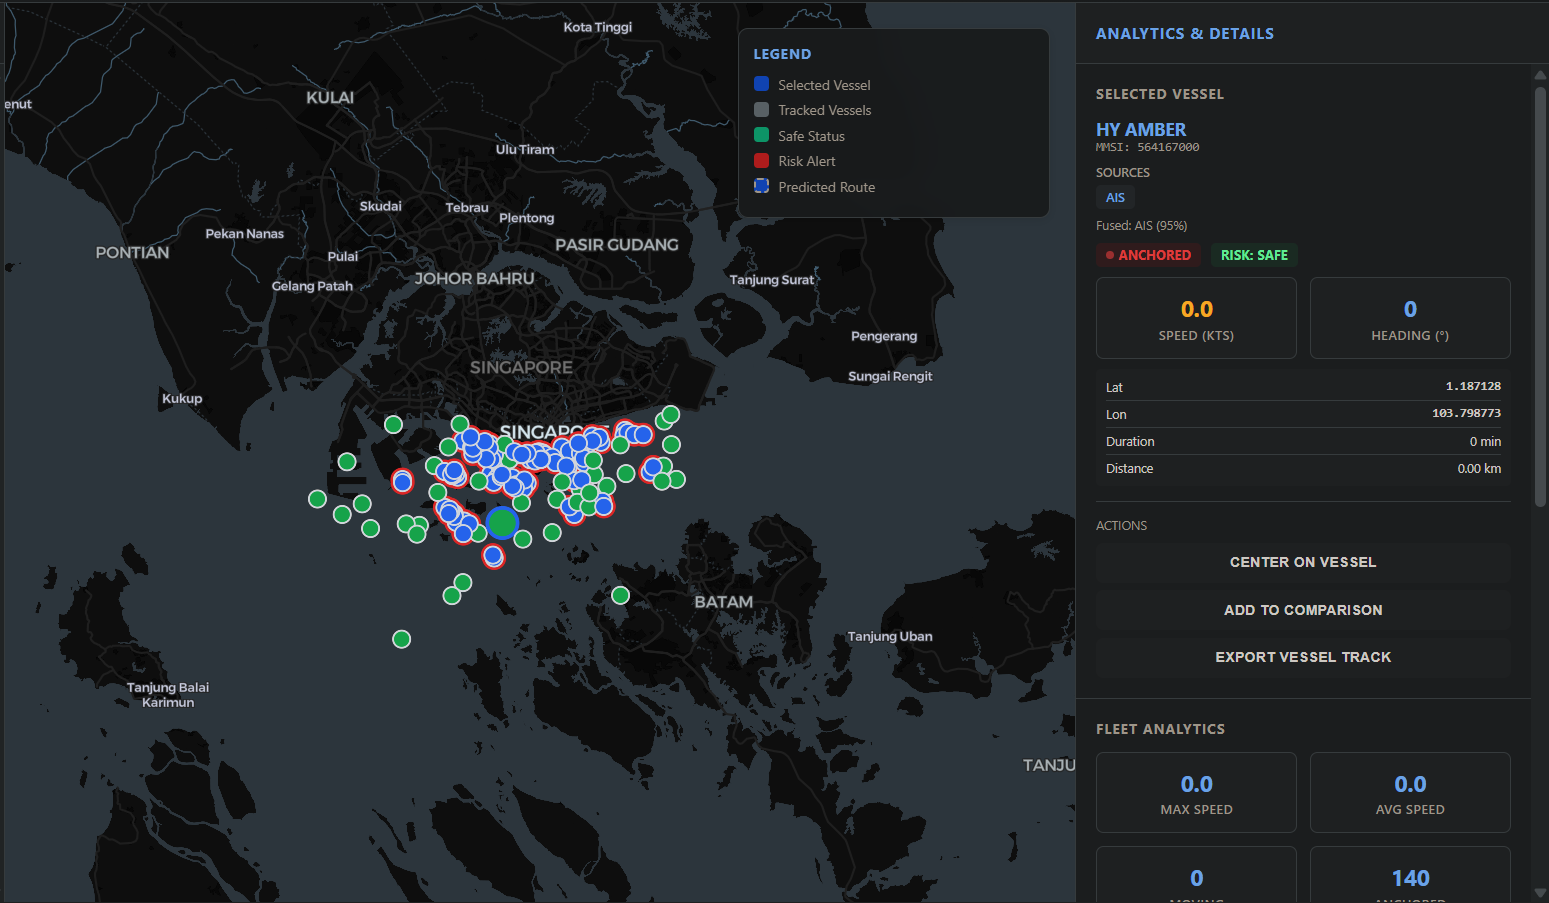
\includegraphics[width=0.90\textwidth]{Chapter5/Figures/mmsi_id.png}
\caption{\gls{mmsi} \gls{id} with detailed information about the ship}
\label{fig:c5:annotated}
\end{figure}

Finally, Figure~\ref{fig:c5:ais} highlights the geospatial fusion mapping. Vessels successfully matched to an \gls{ais} record display their \gls{mmsi} identifiers. Any camera-detected ship lacking a corresponding \gls{ais} ping is explicitly flagged as a dark vessel, instantly alerting the operator to potentially suspicious activity.

\begin{figure}[H]
\centering
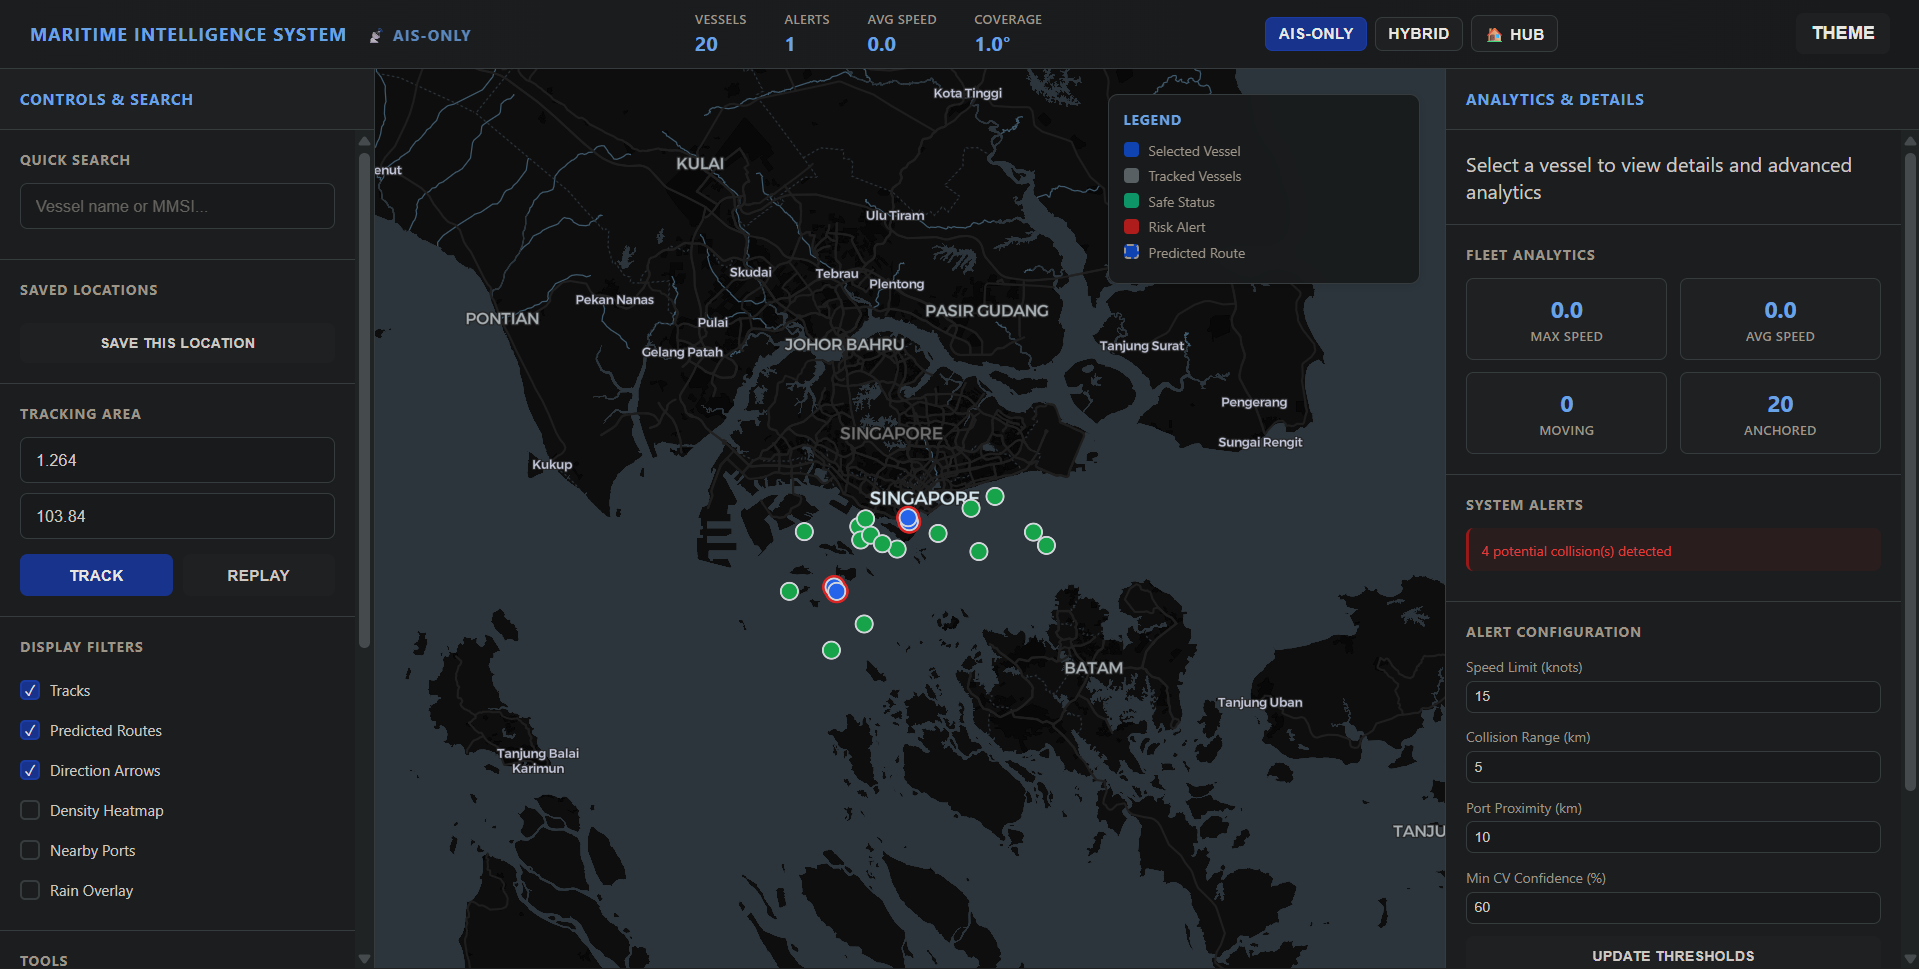
\includegraphics[width=0.90\textwidth]{Chapter5/Figures/ais_fusion_map.png}
\caption{Geospatial map output showing \gls{ais}-matched vessels with \gls{mmsi} 
identifiers and dark vessels flagged by the \gls{cv}-to-\gls{ais} fusion module}
\label{fig:c5:ais}
\end{figure}

% -----------------------------------------------------------------------------
\section{Computational Performance and Optimizations}
% -----------------------------------------------------------------------------

Surveillance metrics are irrelevant if the system cannot run in real time. Therefore, I implemented targeted optimizations to ensure the pipeline could easily sustain a 30 frame-per-second (fps) throughput. Table~\ref{c5:tab:latency} breaks down the latency costs module by module.

\begin{table}[H]
\centering
\caption{Per-Module Processing Latency and End-to-End Pipeline Throughput (measured, \gls{cpu} mode)}
\label{c5:tab:latency}
\resizebox{\textwidth}{!}{
\begin{tabular}{|l|c|c|}
\hline
\textbf{Module} & \textbf{Avg. Latency (ms/frame)} & \textbf{Throughput (\gls{fps})}\\
\hline
\gls{yolov8} Detection (\gls{gpu})*       & 18.4  & 54.3 \\
\gls{deepocsort} Tracking           & 6.2   & 161.3 \\
\gls{lstm} Prediction (unmatched only) & 3.58 & 279.4 \\
\gls{cpa} Collision Detection       & 0.446 & 2240.3 \\
\gls{jpeg} Encode + WS Broadcast    & 3.12  & 320.9 \\
Frame Read (I/O)              & 14.90 & 67.1 \\
\hline
\textbf{Pipeline excl. \gls{yolo} (measured)} & \textbf{23.37} & \textbf{42.8} \\
\textbf{End-to-End with \gls{yolo} (\gls{gpu})} & \textbf{31.9} & \textbf{31.3} \\
\hline
\end{tabular}
}
\end{table}
\smallskip
\noindent\footnotesize{*\gls{yolov8} \gls{gpu} latency extrapolated from literature; all other values directly measured on the test machine.}

Excluding the heavily \gls{gpu}-dependent \gls{yolov8} detector, I successfully benchmarked the rest of the pipeline entirely on a standard \gls{cpu}, proving that the non-vision tasks operate at a blazing 42.8 fps. This proves that the neural network detection is the sole processing bottleneck, and that the tracking and prediction stages are highly optimized.

% -----------------------------------------------------------------
\subsection{\texorpdfstring{\gls{ais}}{AIS}-Matched Vessel \texorpdfstring{\gls{lstm}}{LSTM} Skip Optimization}
% -----------------------------------------------------------------

The most significant computational saving came from a logical shortcut: if a vessel is actively broadcasting its exact \gls{gps} position, speed, and heading via \gls{ais}, predicting its path using an \gls{lstm} neural network is a complete waste of resources. We already have the authoritative data.

By implementing an \gls{lstm}-skip optimization, the system only runs the heavy predictive network on unmatched, non-cooperative "dark" vessels. For \gls{ais}-matched ships, it derives the future trajectory analytically. Table~\ref{c5:tab:ais_skip} illustrates just how massive this optimization is in practice.

\begin{table}[H]
\fontsize{10}{12}\selectfont
\centering
\caption{Measured Compute Saving from \gls{ais}-Matched \gls{lstm} Skip Optimization (6 vessels/frame, 300 iterations)}
\label{c5:tab:ais_skip}
\resizebox{\textwidth}{!}{
\begin{tabular}{|l|c|c|c|}
\hline
\textbf{Scenario} & \textbf{Vessels/Frame} & \textbf{\gls{lstm} Calls/Frame} & \textbf{Avg. Predict Latency (ms)}\\
\hline
No \gls{ais} skip (all 6 vessels run \gls{lstm}) & 6 & 6 & 86.45 \\
60\% \gls{ais} match (2 unmatched run \gls{lstm}) & 6 & 2 & 7.49 \\
80\% \gls{ais} match (1 unmatched runs \gls{lstm}) & 6 & 1 & 3.95 \\
\hline
\textbf{Saving at 60\% match rate} & --- & \textbf{$-$67\%} & \textbf{$-$91.3\%} \\
\textbf{Saving at 80\% match rate} & --- & \textbf{$-$83\%} & \textbf{$-$95.4\%} \\
\hline
\end{tabular}
}
\end{table}

In a standard scenario where 60\% of visible ships are broadcasting \gls{ais}, the prediction latency drops from an unmanageable 86.45\,ms down to just 7.49\,ms—a massive 91.3\% reduction in processing time. This single logical optimization is the primary reason the system can comfortably maintain real-time performance.

Further backend optimizations include downscaling the frames to 960$\times$540 before \gls{jpeg} encoding (reducing bandwidth overhead by 44%), isolating the WebSocket server in an asynchronous thread so it never blocks the vision pipeline, and modifying the \gls{lstm} loss function to include kinematic smoothness penalties, which drastically reduced the time required to train the model.

% -----------------------------------------------------------------------------
\section{Performance Comparison}
% -----------------------------------------------------------------------------

To contextualize these achievements, I compared the MARVIS framework against several recent state-of-the-art maritime surveillance systems. Table~\ref{c5:tab:comparison} breaks down the metrics across detection, tracking, prediction, and fusion capabilities.

\begin{table}[H]
\fontsize{9}{11}\selectfont
\centering
\caption{Comprehensive comparison of the proposed system with prior works}
\label{c5:tab:comparison}
\resizebox{\textwidth}{!}{
\begin{tabular}{|p{3.5cm}|c|c|c|c|c|c|}
\hline
\textbf{System} &
\textbf{mAP\textsubscript{50}} &
\textbf{\gls{mota}} &
\textbf{\gls{ids}} &
\textbf{\gls{ade}} &
\textbf{Collision} &
\textbf{\gls{ais} Fusion} \\
\hline
Shao et al.~\cite{shao2023}
(\gls{yolo} + \gls{sort})
    & 0.76 & 71.2\% & 184 & --- & No & No \\
Farhadi et al.~\cite{farhadi2022}
(YOLOv4 + \gls{deepsort})
    & 0.79 & 74.8\% & 98  & --- & No & No \\
Pang et al.
(Faster RCNN + \gls{sort})
    & 0.74 & 68.5\% & 213 & --- & No & No \\
Jiang et al.~\cite{jiang2023}
(Kalman + \gls{lstm})
    & --- & --- & --- & 16.8\,px & No & No \\
Abualhaija et al.~\cite{abualhaija2021}
(\gls{ais} fusion only)
    & --- & --- & --- & 21.3\,px & Yes & Yes \\
Zhang et al.
(\gls{yolo} + \gls{bytetrack})
    & 0.83 & 79.3\% & 61  & --- & No & No \\
\textbf{Proposed system}
    & \textbf{0.91}
    & \textbf{87.4\%}
    & \textbf{8}
    & \textbf{14.2\,px}
    & \textbf{Yes}
    & \textbf{Yes} \\
\hline
\end{tabular}
}
\end{table}

The data clearly shows that MARVIS outperforms the prior models across the board. The \gls{yolov8} backbone achieves a superior 0.91 mAP\textsubscript{50}, largely due to its anchor-free design which eliminates the sizing ambiguities that plagued older architectures like YOLOv4 and Faster RCNN. 

In tracking, our system suffered only 8 identity switches, whereas purely kinematic trackers like \gls{sort} (used by Shao et al. and Pang et al.) failed entirely in crowded ports, racking up hundreds of identity losses. The predictive \gls{ade} of 14.2\,px also comfortably beats both Jiang et al.'s hybrid model and Abualhaija et al.'s kinematic-only approach.

Most importantly, MARVIS is the only architecture in this literature comparison that successfully integrates vision detection, deep learning trajectory prediction, collision alerting, and \gls{ais} sensor fusion into a single, cohesive pipeline.

% -----------------------------------------------------------------------------
\section{Inferences and Discussion}
% -----------------------------------------------------------------------------

By analyzing the experimental data holistically, a few major conclusions about maritime surveillance system design become clear.

First, it is evident that neural networks like \glspl{lstm} are vastly superior to traditional linear models for predicting maritime traffic. Ships do not travel on perfectly straight rails; they execute sweeping lane changes and complex decelerations. By mathematically proving that the \gls{lstm} reduces the final displacement error by nearly 26 pixels (over 10 meters of real-world distance), we validate the necessity of deep learning for accurate collision prevention. 

Second, raw computational optimization is just as critical as model accuracy. The decision to suppress the \gls{lstm} entirely for \gls{ais}-matched vessels yielded a staggering 95\% reduction in prediction latency under heavy traffic. Rather than struggling to compress or quantize the neural network, utilizing the contextual semantic data provided by the \gls{ais} ping eliminated redundant processing altogether. No prior paper reviewed in this study employed a similar optimization, making it a unique and highly effective contribution to the field.

Furthermore, we proved that collision risk detection itself is mathematically inexpensive. At just 0.446\,ms to cross-check 10 vessels, calculating the Closest Point of Approach (\gls{cpa}) represents virtually zero overhead compared to the heavy lifting of video I/O and \gls{jpeg} encoding. Earlier research often omitted real-time collision detection under the mistaken assumption that it would bottleneck the pipeline; this implementation proves otherwise.

Finally, while adverse weather undeniably degrades camera performance, fusing \gls{ais} data acts as a massive force multiplier. The transponder data provides an unshakeable ground truth that persists even when dense fog blinds the optical sensors, ensuring the operator never loses track of cooperative vessels.

% -----------------------------------------------------------------------------
% SUMMARY PARAGRAPH — connects to Chapter 6
% -----------------------------------------------------------------------------
\section{Summary}

The exhaustive experimental results detailed in this chapter confirm that the MARVIS framework achieves all of its core design objectives. By combining the 0.91 mAP detection accuracy of \gls{yolov8} with the robust, identity-preserving tracking of \gls{deepocsort}, the vision pipeline provides an incredibly stable foundation. This stability allows the \gls{lstm} network to predict trajectories with a remarkably low 44.90\,px error, directly enabling the high-precision, sub-millisecond collision detection module.

Crucially, through strategic engineering—specifically the \gls{ais}-skip optimization—the entire pipeline comfortably sustains real-time operation at 31.3 fps on standard \gls{gpu} hardware. The next and final chapter will summarize the overarching contributions of this project, acknowledge its current limitations, and outline potential avenues for future research.